\documentclass[12pt]{article}
\usepackage[utf8]{inputenc}
\usepackage[margin=1.2in]{geometry}
\usepackage{amsmath, amssymb, amsthm, graphicx, float}
\usepackage{subfig, subfloat}
\allowdisplaybreaks
\title{Competition 2}
\author{CS 4786\\
Cornell University\\
Team Name - Thug Life}


\renewcommand{\P}{\ensuremath{\textup{\textbf{P}}}}

\newcommand{\E}{\ensuremath{\textup{\textbf{E}}}}

\DeclareMathOperator*{\argmaxA}{arg\,max}

\begin{document}

\maketitle
\setlength{\parindent}{0pt}

\section*{Introduction}


All of our experiments were conducted in MATLAB using the Statistics and Machine Learning Toolbox functions related to hidden Markov Models, namely, \verb|hmmtrain| and \verb|hmmdecode|. 

\section*{Choosing number of states}
One of the most important task for doing accurate prediction of missing samples is to get the best estimate of the underlying Hidden Markov Model. And to get the best estimate of the underlying HMM it is very important to choose the number of states in the Markov Model correctly. \\ 
\\
HMM is defined by the following parameters, $\theta$:
\begin{itemize}
    \item Number of possible states (S)
    \item State Transition Matrix
    \item Emission Matrix
    \item Prior on the starting state
\end{itemize}

We are mostly interested in estimating the first three parameters of the HMM. If we know the number of states (S), we can use the Baum-Welch algorithm to estimate the other parameters. We used Matlab's library implementation of Baum-Welch algorithm to learn the parameters from data. The library function we used was \verb|hmmtrain|. \\
\\
Instead of just randomly guessing and trying the various possible values for S, we decided to use a more principled way. We decided to sweep the values of S over the range 1 to 11 and performed k-fold cross validation to pick the best S. Best S is the one which has the maximum likelihood over the validation set given the parameters of HMM (which we learn from training set). \\
\\
We used the first 100 rows of the data matrix given to us for this experiment. So our dataset D = \{First 100 rows of file fillindata.csv\}. Below are the steps we performed to find S:
\begin{itemize}
    \item Set K=10
    \item For fold 1 to K
    \begin{itemize}
        \item Split D into training and validation set
        \item Train on training set, using Baum-Welch (\verb|hmmtrain|). This step gives us $\theta$ for this fold.
        \item Calculate the likelihood of validation set given the $\theta$ estimated in previous step. We used Matlab function \verb|hmmdecode|, which implements Forward-Backward algorithm, to get the likelihood.
    \end{itemize}
    \item end For
    \item Average over the likelihood of all the folds.
    
\end{itemize}


The above algorithm is repeated with different values of S. Below we show the results we obtained with this experiment which guided us to choose the values of S, the \# of states in our HMM model.\\
\\
Figures 1 \& 2 show the table \& plot resp. with the k-fold cross validation likelihood values we get across different values of S. 

\begin{figure}[H]
\centering
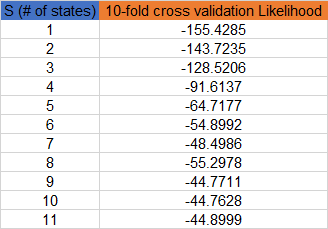
\includegraphics[width=10cm]{table2.png}
\caption{k-fold cross validation table across different values of S}
\label{Fig1: k-fold cross validation table across different values of S}
\end{figure}

\begin{figure}[H]
\centering
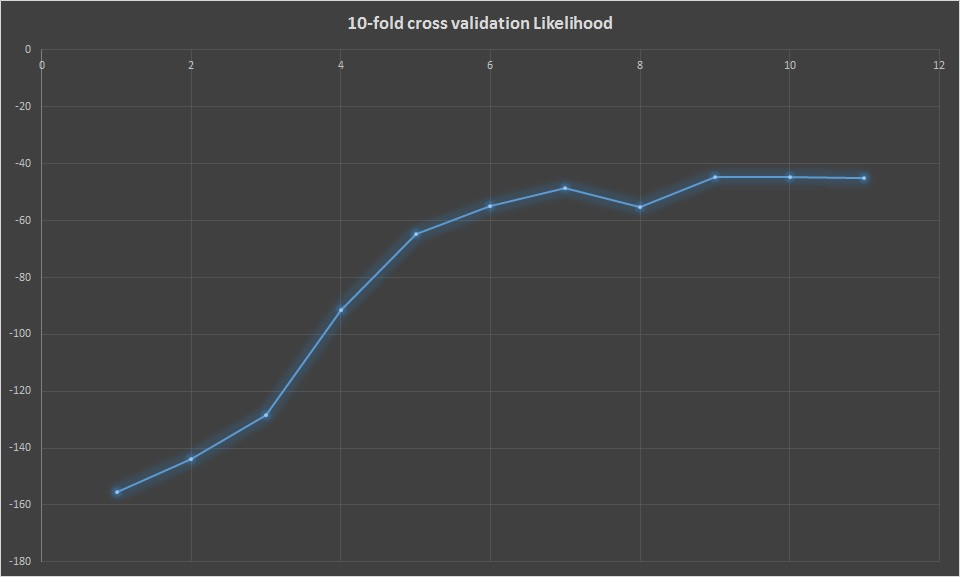
\includegraphics[width=14cm]{sweepPlot2.jpg}
\caption{k-fold cross validation plot across different values of S}
\label{Fig1: k-fold cross validation plot across different values of S}
\end{figure}

From the above figures we can see that the best value for \# of states is \textbf{10}. We can also see that S= 9, 10, 11 all perform equally well, so it looks like that the correct number of states is 10 and any \# of states above that is sufficient to correctly fit the data. We chose 10 because there is no good reason to choose more states. On the other hand, it might overfit if we choose more states than required.\\ 
\\
Below we show the Transition matrix and the emission matrix for S=9 case.\\

\textbf{Transition Matrix}

\begin{center}
\begin{tabular}{|c c c c c c c c c|}
    0.0913    &0.0154    &0.8855    &0.0000     &    0    &0.0000    &0.0000    &0.0000    &0.0078\\
    0.9095    &0.0466    &0.0000    &     0    &0.0000    &0.0000    &0.0000    &     0    &0.0439\\
    0.0002    &0.0018    &0.0649    &0.0000    &0.0000    &0.0000    &0.9121    &0.0000    &0.0210\\
    0.0000    &0.0153    &     0    &0.0074    &0.9526    &0.0004    &0.0000    &0.0057    &0.0187\\
    0.0000    &0.0159    &     0    &0.0000    &0.0383    &0.9432    &     0    &0.0000    &0.0027\\
    0.0000    &0.6462    &0.0000    &0.0000    &0.0001    &0.1133    &     0    &0.0000    &0.2403\\
    0.0000    &0.0047    &0.0000    &0.7260    &0.0000    &0.0018    &0.0733    &0.1740    &0.0202\\
    0.0000    &0.0027    &     0    &0.2709    &0.6631    &0.0005    &0.0000    &0.0591    &0.0037\\
    0.8830    &0.0886    &0.0000    &     0    &0.0000    &0.0000    &0.0000    &     0    &0.0284\\
\end{tabular}
\end{center}\\

\\
\textbf{Emission Matrix}

\begin{center}
\begin{tabular}{|c c c c c|}
    0.9432    &0.0568    &0.0000    &     0    &0.0000 \\
    1.0000    &0.0000    &0.0000    &     0    &0.0000 \\
    0.0000    &0.9520    &0.0480    &0.0000    &    0 \\
    0.0000    &     0    &0.0000    &0.9541    &0.0459 \\
    0.0000    &     0    &     0    &0.0030    &0.9970 \\
    0.0479    &     0    &0.0000    &0.0000    &0.9521 \\
    0.0000    &0.0000    &0.9601    &0.0399    &0.0000 \\
    0.0000    &     0    &0.0002    &0.9398    &0.0601 \\
    1.0000    &0.0000    &0.0000    &0.0000    &0.0000 \\
\end{tabular}
\end{center}

\section*{Predicting missing values}
\subsection*{Method 1 - Maximum Likelihood}

We first estimate the transition and emission probabilities with the 10 states using Baum-Welch algorithm on the 100 sequences with complete observation given to us. We used \verb|hmmtrain| command on Matlab for this. The initialization we did for initial guesses for transition and emission probabilities was random, but we make sure that the initial guess for transition matrix and emission matrix are stochastic i.e. the rows sums up to 1. After the training converged, we used the estimated transition and emission probabilities, $\theta$, to predict the missing values in the sequences. For predicting, we use maximum likelihood criterion i.e. we plug in all 5 values the missing sample can take in each sequence and estimate the likelihood. We then pick the value that resulted in the highest likelihood. This is repeated for all the 900 sequences which has a missing element. To estimate the likelihood we used Forward-Backward algorithm implementation in Matlab toolbox.\\
\\
More formally,
\begin{align*}
Y_{i} &= \argmaxA_{y \ \in \ \{1,2,3,4,5\} } P(x_{1}, x_{2}, \dots , x_{i-1}, y, x_{i+1}, \dots , x_{100} \ | \ \theta) \\
&= \argmaxA_{y \ \in \  \{1,2,3,4,5\} } P(sequence\ with\ y  \ | \ \theta) 
\end{align*}
where $\theta$ are the parameters of HMM.\\
\\
We repeat this for all 900 sequences and get our predictions. This can be done using  \verb|hmmdecode| command on Matlab for individual sequences. \verb|hmmdecode| returns the log-likelihood, but it works for us since log preserves the ordering. This submission gave us a score of \textbf{0.9111}, which is $3^{rd}$ best on the Kaggle leaderboard.

\subsection*{Method 2 - Different initialization seed}

We once again tried the same method as before but with a different initialization seed. The motivation for this was that we may converge to a different local minima for Baum-Welch algorithm, which could possibly be better than the previous one. We compared the predictions from this method with the previous one and observed that 22 predictions were different. On perusing these sequences, we noticed that predictions from both these methods seemed reasonable on these 22 sequences. We went ahead and made a submission with these new predictions. This submission gave us a score of \textbf{0.90}.

\subsection*{Method 3 - Training on full data}

We then performed training on all the 1000 sequences. The missing values were filled with the predictions that were made from Method 1. After obtaining the transition and emission probabilities, we performed prediction on the 900 sequences. This submission gave us a score of \textbf{0.89556}.

\subsection*{Method 4 - Predictions from Method 1 + Manual supervison}

We once again used the predictions from method 1. We noticed that for few sequences there were two observation values that had almost the same log-likelihood. In such cases, we picked the sample value corresponding to $2^{nd}$ best log-likelihood and made that our prediction. For example, for the sequence 266, we noticed that 2 and 3 had similar log-likelihood values and which were much higher compared to the other values. But 3 was the higher of the two. So we pick 2 as our prediction. We repeated this for all such cases. This submission gave us a score of \textbf{0.9022}

\subsection*{Method 5 - Experiments with different \# of states S}

To solidify our intuition from the graph that prediction accuracy correlates with the likelihood as shown in figures 1 and 2, we trained and tested a few models with different states. The table below summarizes the results. 

\begin{center}
\begin{tabular}{|c|c|}
\hline
\textbf{\# of states}     & \textbf{Prediction score} \\ \hline
6   & 0.7911        \\ \hline
7   & 0.9044        \\ \hline
8   & NA            \\ \hline
9   & 0.9111        \\ \hline
10  & 0.9111        \\ \hline
11  & 0.9088        \\ \hline
12  & 0.9088        \\ \hline
\end{tabular}
\end{center}
\\
We therefore did not explore S=8 as we see a dip at that point in figure 2. 

\section*{Accounting for reversed sequences}
For all of our experiments, we did not account for reversed sequences but still got a score of around \textbf{ 0.90}. We did try to find reversed sequences by looking at the log-likelihood values of predicted sequences. Sequences with log-likelihood values lower than usual could be considered to be outliers (which in this case are reversed sequences). 

\section*{Parameters for our best performing model}

No. of states       = 10 \\
Tolerance           = 1e-4 \\
No. of observations = 5 (given)\\
\\
Predictions were made as explained in method 1. 

\section*{Comments}
For all the algorithms we used like Baum-Welch (\verb|hmmtrain|) or Forward-Backward (\verb|hmmdecode|), there were hyper-parameters like the max-iterations, tolerance for convergence criterion, etc. We played around a bit with all these hyper-parameters to find the best combination and then we kept them same over all the experiments we have mentioned in this report. By best combination we mean to choose the hyper-parameters such that the training is not prone to overfitting. For example, we reduced the tolerance in \verb|hmmtrain| which governs the convergence criteria of Baum-Welch algorithm, from default 1e-6 to 1e-4, so that it is less prone to overfit.

\section*{Conclusion}
We got our best accuracy with Method 1 which we believe is the most principled way for this prediction task. We think that choosing the \# of States was an interesting task which helped us significantly in our predictions. One other aspect to the problem was the starting point of Baum-Welch algorithm which can land you into different local minima. So we tried a few different initial guesses. Though the algorithm converged at different local minima, the predictions were very similar which indicates that most of these local minima were equally good. 

\end{document}
